
%%%%%%%%%%%%%%%%%
%%%%%%%%%%%%%%%%%
\begin{frame}
	\shiftedframetitle{3. Implementation}
%\begin{minipage}{0.35\textwidth}
\begin{itemize}
\item<1->[]
\begin{tcolorbox}[title= \textbf{Domain Mapping},colframe=TUMDarkBlue] 
\begin{table}[]
\begin{tabular}{llp{2cm}ll}
\textbf{1.} Supercritical & $2D$ SWE  $\rightarrow$  $2D$  SWE  & & \textbf{5.} Supercritical & $3D$ OF   $\rightarrow$  $2D$ SWE  \\ 
\textbf{2.} Subcritical   & $2D$ SWE  $\rightarrow$  $2D$  SWE & & \textbf{6.} Subcritical   & $3D$ OF   $\rightarrow$  $2D$ SWE     \\[0.2cm]
\textbf{3.} Supercritical & $2D$ SWE  $\rightarrow$  $3D$  OF   & & \textbf{7.} Supercritical & $3D$ OF   $\rightarrow$  $3D$ OF    \\ 
\textbf{4.} Subcritical   & $2D$ SWE  $\rightarrow$  $3D$  OF & & \textbf{8.} Subcritical   & $3D$ OF   $\rightarrow$  $3D$ OF
\end{tabular}
%\caption{Mapping setups}
%\label{table:1}
\end{table}
\end{tcolorbox}
%\end{minipage}
%\hspace{1cm}\\
%\begin{minipage}{.55\textwidth}
%\addtolength{\leftmargini}{-0.8cm}
%\begin{itemize}
\vspace{0.5cm}
\item<2->[]
\begin{tcolorbox}[title= \textbf{Scenarios}, colframe=TUMDarkBlue] 
\begin{table}[!h]
\centering
\begin{tabular}{l|ll|ll}
 & {\large \textbf{Supercritical}} & & {\large \textbf{Subcritical}} &\\[0.3cm]
\textbf{Case / Domain} & \textbf{Left domain} & \textbf{Right domain} & \textbf{Left domain} & \textbf{Right domain}\\[0.3cm]
\textbf{SWE $\rightarrow$ SWE} & Radial breaking dam      & Surface at rest   & Radial breaking dam      & Radial breaking dam     \\[0.1cm]
\textbf{SWE $\rightarrow$ OF}  & Radial breaking dam x2   & Surface at rest & Flow to the right & Surface at rest with wall     \\[0.1cm]
\textbf{OF $\rightarrow$ SWE}  & Radial breaking dam   & Surface at rest & Flow to the right & Surface at rest with wall   \\[0.1cm]
\textbf{OF $\rightarrow$ OF}   & Breaking dam      & Empty domain & Breaking dam      & Empty domain with wall
\end{tabular}
%\caption{Scenarios for each setup on supercritical flow.}
%\label{t:condsSup}
\end{table}
\end{tcolorbox}
%\item<3->[]
%\begin{tcolorbox}[title= \textbf{Subcritical Cases}, colframe=TUMDarkBlue,
%colback=TUMDarkBlue!30]
%\begin{table}[!h]
%\centering
%\begin{tabular}{lll}
%\textbf{Case / Domain} & \textbf{Left domain} & \textbf{Right domain} \\[0.3cm]
%\textbf{SWE $\rightarrow$ SWE} & Radial breaking dam      & Radial breaking dam      \\[0.1cm]
%\textbf{SWE $\rightarrow$ OF}  & Flow to the right & Surface at rest with wall        \\ [0.1cm]
%\textbf{OF $\rightarrow$ SWE}  & Flow to the right & Surface at rest with wall      \\[0.1cm]
%\textbf{OF $\rightarrow$ OF}   & Breaking dam      & Empty domain with wall
%\end{tabular}
%%\caption{Scenarios for each setup on subcritical flow.}
%%\label{t:condsSub}
%\end{table}
%\end{tcolorbox}

%\end{itemize}
%\end{minipage}
\end{itemize}
\end{frame}


\begin{frame}
%TODO improve this slide
\shiftedframetitle{3. Implementation}
\begin{table}[!ht]
%\hspace{7cm}
\centering
\begin{tabular}{ccc}
\textbf{Boundary Conditions} & & \\
\hline
                    				  &$ h$ and $q$ on $\Gamma_{2D}$ & $\alpha, p$ and $u$ on $\Gamma_{3D}$ \\ \hline
%Supercritical \& Subcritical \case{SWE}{SWE}  & $\begin{aligned}[t] h_{left} &= h_{left} + \partial{h}/\partial{n} \\  hu_{left} &= hu_{left} + \partial{hu}/\partial{n}\\  hv_{left} &= hv_{left} + \partial{hv}/\partial{n} \end{aligned}$ &                  \\ \hline
%% Subcritical \case{SWE}{SWE}  & $\begin{aligned}[t] \qquad h_{left} = h_{left} + \partial{h}/\partial{n} \end{aligned}$ &                  \\ \hline
\myTUMdarkblue{Supercritical} \myTUMdarkblue{SWE $\rightarrow$ OF}  & $\begin{aligned}[t] \myTUMdarkblue{\partial{h}/\partial{n} = 0} \\ \myTUMdarkblue{\partial{q}/\partial{n} = 0} \end{aligned}$                 &  $\begin{aligned}[t] \myTUMdarkblue{\alpha = f(h)} \\ \myTUMdarkblue{\partial{p}/\partial{n} = 0}  \\ \myTUMdarkblue{u = f(q,u)}   \end{aligned}$   \\ \hline
Subcritical \case{SWE}{OF}  & $\begin{aligned}[t] h = \hthD \\ \partial{q}/\partial{n} = 0 \end{aligned}$&    $\begin{aligned}[t] \partial{\alpha}/\partial{n} = 0 \\ \partial{p}/\partial{n} = 0 \\ u = f(q,u) \end{aligned}$              \\ \hline
Supercritical   \case{OF}{OF}  &$\begin{aligned}[t] h=\hthD \\ q=\qthD \end{aligned}$                                  & $\begin{aligned}[t] \partial{\alpha}/\partial{n} = 0 \\ \partial{p}/\partial{n} = 0 \\ \partial{u}/\partial{n} = 0 \end{aligned}$                      \\ \hline
Subcritical  \case{OF}{SWE} & $\begin{aligned}[t] \partial{h}/\partial{n} = 0 \\ q=\qthD \end{aligned}$                 &  $\begin{aligned}[t] \partial{\alpha}/\partial{n} = 0 \\ p = f(h) \\ \partial{u}/\partial{n} = 0 \end{aligned}$                \\ \hline
Supercritical  \case{OF}{OF} &   &  $\begin{aligned}[t] \alpha_{right} = \alpha_{left} \\ u_{right} = u_{left} \\ p_{left} = p_{right} \end{aligned}$                \\ \hline
%Subcritical   \case{OF}{OF}  & &     \textit{discussion in Section \ref{sec:resultsOFOF}}   \\ \hline
\end{tabular}
%\caption{Dirichlet and Neumann boundary conditions for the inter-dimensional combinations and flow characterization \cite{mintgen}, and for the cases on the same dimension.}
\end{table}


%\begin{figure}
%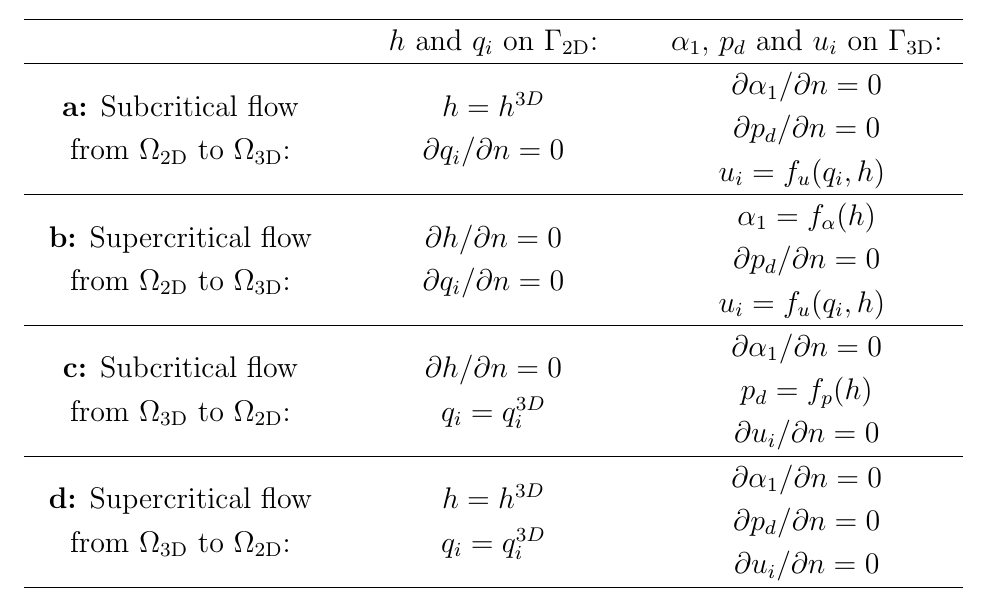
\includegraphics[scale=0.43]{Resources/Images/bcs_mintgen.png}
%\caption{Boundary conditions \cite{mintgen}}
%\end{figure}
\end{frame}

